\documentclass[tikz]{standalone}

%\usepackage{etoolbox}
\usepackage{fontspec}
\setmainfont[Ligatures=TeX, Mapping=tex-text]{Lato}
%\usepackage[default]{lato}
\usepackage{unicode-math}
%\setmathfont{Lete Sans Math}
\setmathfont{LeteSansMath.otf}
%\usepackage{lete-sans-math}
\usepackage{tikz}
\usetikzlibrary{math}
\usepackage{xfp}

\begin{document}
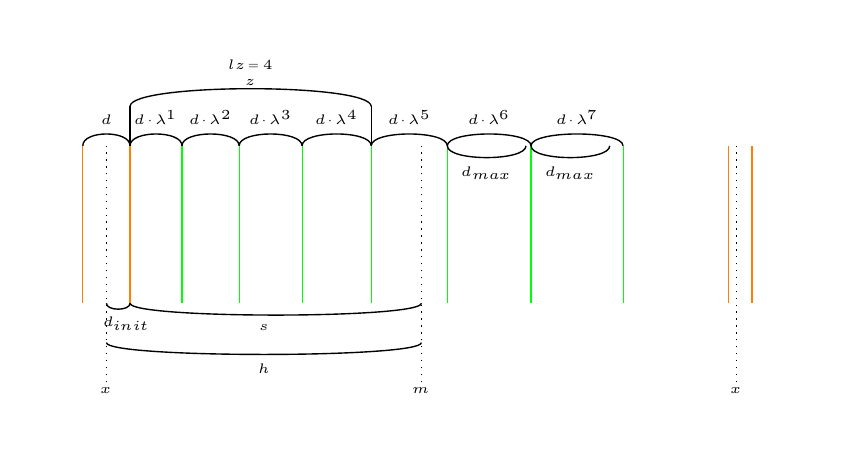
\begin{tikzpicture}

\def\width{10}
\def\height{5}
\def\ox{\fpeval{\width /2}}
\def\oy{\fpeval{\height /2}}
\coordinate (O) at (\ox,\oy);

\tiny
\path [use as bounding box] (0,0) rectangle (\width,\height);

% SHAPE
%\filldraw [line width=0.5pt, fill=orange] (\ox,\oy)
%	+(-0.5,-0.5) node[draw, fill=black, circle, inner sep=1pt] {} node[below left] {0} --
%	+(0.5,-0.5) node[draw, fill=black, circle, inner sep=1pt] {} node[below right] {1} --
%	+(0.5,0.5) node[draw, fill=black, circle, inner sep=1pt] {} node[above right] {2} --
%	+(-0.5,0.5) node[draw, fill=black, circle, inner sep=1pt] {} node[above left] {3} --
%	cycle;

% PORTS
%\draw [line width=2pt] (\ox,\oy) ++(-0.5,0) node[right] {1} +(0,-0.5) -- +(0,0.5);
%\draw [line width=2pt] (\ox,\oy) ++(0,-0.5) node[above] {2} +(-0.5,0) -- +(0.5,0);



% MID LINE
\draw [line width=0.5pt, dotted] (O) +(0,-2) node[below] {$m$} -- +(0,1);

% EDGE LINES
\draw [line width=0.5pt, dotted] (\ox,\oy) +(-4,-2) node[below] {$x$} -- +(-4,1);
\draw [line width=0.5pt, dotted] (\ox,\oy) +(4,-2) node[below] {$x$} -- +(4,1);

% POLICY LINES
%\draw [line width=0.5pt, orange] (\ox,\oy) ++(-4,0)
%	+(-0.2,-1) -- +(-0.2,1)
%	+(0.2,-1) -- +(0.2,1);
%\draw [line width=0.5pt, orange] (\ox,\oy) ++(4,0)
%	+(-0.1,-1) -- +(-0.1,1)
%	+(0.2,-1) -- +(0.2,1);
% Function: policy line
% #1 : x
% #2 : x1 (relative to x)
% #3 : x2 (relative to x)
\newcommand{\policylines}[3]{%
	\draw [line width=0.5pt, orange] (\ox,\oy) ++(#1,0)
		+(#2,-1) -- +(#2,1)
		+(#3,-1) -- +(#3,1)%
}
\policylines{-4}{-0.3}{0.3}; % 1/2 - Halfs rule
\policylines{4}{-0.1}{0.2}; % 1/3 - Thirds rule

% LINES
%\newcommand{\drawline}[2][violet]{%
%	\draw [line width=0.5pt, color={#1}] (\ox,\oy)
%		+(#2,-1) -- +(#2,1)%
%}
%\drawline[orange]{3};
%\newcommand{\drawline}[2][violet]{%
%	\draw [line width=0.5pt, {#1}] (\ox,\oy)
\newcommand{\drawline}[2][line width=0.5pt, color=black]{%
	\draw [{#1}] (\ox,\oy)
		+(#2,-1) -- +(#2,1)%
}
%\drawline[orange, dotted]{3};
%\drawline{2.5};
%
%\draw [line width=0.5pt, violet] (\ox,\oy) ++(-3.7,-1)
%%	++(0,0) +(0,2)
%	++(1.2,0) -- +(0,2)
%	++(2.4,0) -- +(0,2)
%;


% First, produce a list of lines coordinates
% Then, use the list to draw the lines and draw annotations
% https://tex.stackexchange.com/questions/662928/is-this-the-right-way-to-understand-let-def-edef-gdef-xdef-newcommand-ren
% edef daclare a var, performing expansion
% xdef declare a global edef var
\xdef\lines{}
% TODO define as func with args { x, d_init, d, direction }
\foreach \n in {1,...,2} {
	\edef\tmp{\lines,\n}
	\xdef\lines{\tmp}
}

%%%% #1 : output var
%%%% #2 : n
%%%% #3 : x
%%%% #4 : d
%%%% #5 : d_init
%%%% #6 : lambda
%%%% #7 : direction
%%%\newcommand{\createlines}[6] {%
%%%	% ##1 : n
%%%	\newcommand{\calculate}[1] {%
%%%%		\fpeval{#3 + ##1}%
%%%		\fpeval{(#3 + #5) + (#4 * (#6 ^ ##1))}%
%%%	}
%%%	% ##1 : s
%%%	% ##2 : d
%%%	%% ##3 : n
%%%	\newcommand{\calculates}[2] {%
%%%%		\fpeval{#3 + ##1}%
%%%		\fpeval{##1 + (##2 * #6)}%
%%%	}
%%%	\edef\currents{\fpeval{#3 + #5}}
%%%	\edef\currentd{#4}
%%%	\expandafter\xdef\csname #1\endcsname{}
%%%
%%%	\foreach \n in {1,...,#2} {%
%%%		\edef\currentd{\fpeval{\currentd * #6}}
%%%		\edef\currents{\fpeval{\currents + \currentd}}
%%%		\ifnum \n = 1%
%%%%			\edef\tooutput{\calculate{\n}}%
%%%			\edef\tooutput{\currents}%
%%%%			\edef\tooutput{\calculates{\currents}{\currentd}}%
%%%		\else%
%%%%			\edef\tooutput{\csname #1\endcsname,\calculate{\n}}%
%%%			\edef\tooutput{\csname #1\endcsname,\currents}%
%%%%			\edef\tooutput{\csname #1\endcsname,\calculate{\n}}%
%%%		\fi%
%%%		\expandafter\xdef\csname #1\endcsname{\tooutput}%
%%%	}%
%%%}

% #1 : output var
% #2 : n
% #3 : x
% #4 : d
% #5 : d_init
% #6 : lambda
% #7 : direction (+ | -)
\newcommand{\createlines}[7] {%
	\tikzmath{
		real \d, \s;
		\d = #4;
		\s = #3 #7 #5;
		let \ret =;
		for \i in {1,...,#2} {
			\d = \d * #6;
			\s = \s #7 \d;
			if \i == 1
			then { \ret = \s; }
			else { \ret = "\ret,\s"; };
		};
	}
	\expandafter\xdef\csname #1\endcsname{\ret}
}

%\createlines{linus}{3}{-4}
%\createlines{linus}{3}{-4}{0.6}{0.3}{2}
\createlines{lines}{7}{-4}{0.6}{0.3}{1.1}{+}

\edef\orig{\fpeval{-4+0.3}}

\foreach \n [expand list=true, count=\i] in {\lines} {
	\drawline[green]{\n};
%	\draw [line width=0.5pt, red] (\ox,\oy)
%		++(\n,-1) -- +(0,2) node[above] {\n};

%	\draw [line width=0.5pt] (\ox,\oy) ++(-4,0) ++(0.3,0)
	\draw [line width=0.5pt] (\ox,\oy) ++(\orig,0)
		++(0,1) -- +(0,0.5);
	\ifnum \i = 4
		\draw [line width=0.5pt] (\ox,\oy)
			++(\n,1) -- +(0,0.5);
		\draw [line width=0.5pt] (\ox,\oy) ++(0,1.5)
			+(\orig,0)
			.. controls +(0,0.3) and +(0,0.3) ..
			+(\n,0)
			+(\fpeval{(\orig+\n)/2},0.2) node[above] {$z$}
			+(\fpeval{(\orig+\n)/2},0.4) node[above] {$lz=\i$};
	\fi
}

\edef\dmax{1}

\foreach \n [
	expand list=true,
	count=\i,
	remember=\n as \lastn (initially \fpeval{-4+0.3})
] in {\lines} {
	\draw [line width=0.5pt] (\ox,\oy) ++(0,1)
		+(\lastn,0) .. controls +(0,0.2) and +(0,0.2) .. +(\n,0)
		+(\fpeval{(\lastn+\n)/2},0.2) node[above] {$d\cdot\lambda$$^\i$};

	\pgfmathparse{\dmax < \fpeval{abs(\lastn-\n)}}
	\ifnum \pgfmathresult>0
		\draw [line width=0.5pt] (\ox,\oy) ++(0,1)
			++(\lastn,0) .. controls +(0,-0.2) and +(0,-0.2) .. +(\dmax,0)
			+(\fpeval{(\dmax)/2},-0.2) node[below] {$d_{max}$};
	\fi
}



% ANNOTATIONS
\draw [line width=0.5pt] (\ox,\oy) ++(-4,1)
	+(-0.3,0) .. controls +(0,0.2) and +(0,0.2) .. +(0.3,0)
	+(0,0.2) node[above] {$d$};

\draw [line width=0.5pt] (\ox,\oy) ++(-4,-1)
	+(0,0) .. controls +(0,-0.1) and +(0,-0.1) .. +(0.3,0)
	+(0.25,-0.1) node[below] {$d_{init}$};

\draw [line width=0.5pt] (\ox,\oy) ++(0,-1)
	+(-3.7,0) .. controls +(0,-0.2) and +(0,-0.2) .. +(0,0)
	+(-2,-0.2) node[below] {$s$};

%\draw [line width=0.5pt, yellow] (\ox,\oy) ++(0,-1)
%	+(-3.7,0) to [bend right=30] +(0,0)
%	+(-2,-0.2) node[below] {s};

\draw [line width=0.5pt] (\ox,\oy) ++(0,-1.5)
	+(-4,0) .. controls +(0,-0.2) and +(0,-0.2) .. +(0,0)
	+(-2,-0.2) node[below] {$h$};


\end{tikzpicture}
\end{document}
